\styledchapter{Causal Inference}

\section{Rubin Causal Model}



Consider covariates $\left\{X_i\right\}$ and treatment indicators $\left\{W_i\right\}$, along with the response variable $\left\{Y_i\right\}$. The guiding question is: Does $W_i$ ``causally impact'' $Y_i$?

\begin{example}	Let $W_i$ be an indicator for the event that student $i$ received a certificate of merit and $Y_i \in \left\{0,1\right\}$ be an indicator for if student $i$ received a scholarship within a year of the certifications being given out.

	A naive starting point is to conduct a difference-in-means test: considering \[
		\hat{\tau} = \frac{1}{\# \left\{W_i = 1\right\}} \sum\limits_{i: W_i = 1}^{} Y_i - \frac{1}{\# \left\{W_i = 0\right\}} \sum\limits_{i: W_i = 0}^{} Y_i
	,\] 
	if $\hat{\tau}$ is much larger than $0$, we may want to conclude that there is a causal effect of $W_i$ on $Y_i$. 

	However, because confounders like previous academic performance influence both $W_i$ and $Y_i$, we cannot immediately say that the relation is causal.
\end{example}

We want to develop a formal language to talk about causality. While there are many possibility, we will use the potential outcomes framework of Neyman and Rubin.

\begin{definition}[Potential outcomes]
	The potential outcome if $Y_i$ is treated is $Y_i(1)$ and $Y_i(0)$ if $Y_i$ is not treated. 

	For each student, we imagine scenarios in which individual $i$ gets treatment and where they don't get treatment. 
	We link potential outcomes to the observed $Y_i$ by writing \[
		Y_i = \begin{cases}
			Y_i(0), \quad W_i = 0 \\ Y_i(1), \quad W_i = 1
		\end{cases}= W_iY_i + (1-W_i) Y_i
	.\] Implicitly, we are assuming SUTVA.\boxednote{SUTVA stipulates:
	\begin{enumerate}[label=(\roman*)]
		\item Treatment of $i$ only depends on treatment assignment of $i$ and not other observations 
		\item $i$'s potential outcomes are affected by its treatment assignment and treatment, and not those of others
	\end{enumerate}}
\end{definition}

The fundamental challenge of causal inference is that we only see only of the two potential outcomes, and not both.

\begin{definition}[Individual treatment effect]
	The individual treatment effect is \[
		\tau_i = Y_i(1) - Y_i(0)
	.\]
\end{definition}

While we do not know $\tau_i$, we can use it to define estimands of interest.

If we assume $\P\left[W_i = 1\right] \in (0,1)$, then we see \begin{align*}
	\hat{\tau} &= \frac{1}{\# \left\{i: W_i = 1\right\}} \sum\limits_{i: W_i = 1}^{} Y_i - \frac{1}{\# \left\{i: W_i = 0\right\}}\sum\limits_{i:W_i = 0}^{} Y_i\\
			   &\xrightarrow{\P} \E\left[Y_i \mid W_i = 1\right] - \E\left[Y_i \mid W_i = 0\right] \\
			   &= \E\left[Y_i(1) \mid W_i = 1\right] - \E\left[Y_i(0) \mid W_i = 0\right]  \\
			   &= \underbrace{\E\left[Y_i(1) - Y_i\left( 0 \right) \mid W_i = 1\right]}_{ATT}  + \underbrace{\left(\E\left[Y_i(0) \mid W_i = 1\right] - \E\left[Y_i(0) \mid W_i - 0\right]  \right)}_{\text{confounding}} \\
			   &= \underbrace{\E\left[Y_i(1) - Y_i(0) \mid W_i = 0\right]}_{\text{ATU}}+ \left( \E\left[Y_i(1) \mid W_i = 1\right] - \E\left[Y_i(1) \mid W_i = 0\right]  \right)
.\end{align*} 

With the very strong assumption of $W_i \ind \left(Y_i(0), Y_i(1)\right)$, we would have that $\hat{\tau} = \E\left[Y_i(1) - Y_i(0)\right] = ATE$.
Sometimes this orthogonality is enforced by construction; e.g. in RCTs and A/B tests.
However, we often don't have this because of ethical reasons, monetary constraints, or lack of control over treatment assignment in existing datasets (observational studies).

\begin{example}[Regression Discontinuity Design]
	Continuing with the certificate of merit example, consider covariates $X_i \in \left\{1,\ldots,20\right\}$ as test scores that determine $W_i$ by \[
		W_i = \mathds{1}_{X_i > c}, \quad c =10
	.\] 
	We call $X_i$ the \emph{running variable}. The idea of RDD is that students who have $X_i =10$ and students who have $X_j = 11$ are similar and comparable. 
\end{example}

How can we formalize the notion that observations near some cutoff for receiving treatment vs. no treatment are as if they were randomized?
One method is the continuity-based approach. Define the conditional response functions \[
	\mu_{(1)} = \E\left[Y_i(1) \mid X_i = x\right], \quad \mu_{(0)}(x) = \E\left[Y_i(0) \mid X_i = x\right]
.\] 
Can we estimate the average treatment effect $\E\left[Y_i(1) - Y_i(0)\right] $? Only if we assume something like $\E\left[Y_i(1) - Y_i(0) \mid X_i = x\right] $ is constant. 
The causal estimand is the ATE at the cutoff: \[
	\theta = \E\left[Y_i(1) - Y_i(0) \mid X_i = c\right] 
.\] 
We will use nonparametrics to estimate the conditional response functions $\mu_{(1)}(x) := \E\left[Y_i(1) \mid X_i = x\right] $ and $\mu_{\left(0 \right)}(x) := \E\left[Y_i(0) \mid X_i = x\right] $ near the cutoff $c$. We can assume that both $\mu_{(1)}, \mu_{(2)}$ are continuous at $c$,\boxednote{This continuity assumption of $\mu$ at $c$ can be upgraded to something like H\"older continuity.} and as a result, write 
\begin{align*}
	\theta 
	&= \E\left[Y_i(1) - Y_i(0) \mid X_{i} = c\right] \\
	&= \mu_{(1)}(c) - \mu_{(0)}(c) \\
	&= \lim\limits_{x \downarrow c} \mu_{(1)}(x) - \lim\limits_{x \uparrow c} \mu_{(0)}(x)
\end{align*}
with the estimators $\hat{\mu}_{(1)}, \hat{\mu}_{(0)}$ from nonparametric regression.

Estimating the treatment effect at the cutoff with RDD is a bit problematic because we have extra boundary bias.
In practice, we can do local linear regression instead. 

What happens if $X_i$ is discrete? Recall the test scores example: the highest score of any individual in the control group is $9$, which we may consider to be too far from the cutoff score of $10$. There are several ways to deal with this:
\begin{itemize}
	\item We can assume $X_i$ has continuous density at $c$ 
	\item Bias-aware approach: use a continuity assumption to get an upper bound on the possible bias, and widen confidence intervals accordingly. When we assume $\mu_{(1)}(\cdot ) \in \Sigma(1,c)$ but $X_i$ is discrete, we are assuming there exists $\tilde{\mu}_{(1)}$ that is an extension of $\mu_{(1)}(c)$ and in $\Sigma(1,c)$.
\end{itemize}

\section{Estimating Treatment Effects in a RCT}


Consider an RCT in which $W_i \ind \left( X_i, Y_i(0), Y_i(1) \right)$ and $p = \P\left[W_i = 1\right] \in (0,1)$.

Suppose a medication affects one cohort in the population differently than another. The ATE is misleading because it does not capture how treatment affects the different cohorts differently.

We would rather estimate the conditional average treatment effect:\boxednote{By the LIE, we can recover the ATE from the CATEs: \[
	ATE = \E\left[CATE(X_i)\right] 
.\] } \[
	\tau(x) = CATE(x) := \E\left[Y_i(1) - Y_i(0) \mid X_i = x\right]  = \mu_{(1)}(x) - \mu_{(0)}(x)
.\] 
\begin{definition}[$t$-learner]
		For some generic nonparametric method $\mathscr{M}$, we can estimate $\tau(x)$ by\boxednote{The regression method $\mathscr{M}$ may differ between the treatment and control groups, for example if their sample sizes differ sharply.} estimating \[
			\begin{aligned}
				\hat{m}_{(1)} (\cdot ) &= \mathscr{M}\left[ Y_i \sim X_i, i \in \mathscr{D}_1 = \left\{i : W_i = 1\right\} \right], \\
				\hat{m}_{(0)}(\cdot ) &= \mathscr{M}\left[ Y_i \sim X_i: i \in \mathscr{D}_0 = \left\{i: W_i = 0\right\} \right]
			\end{aligned}
		,\] 
	then putting \[
		\tau(x) = \hat{m}_{(1)}(x) - \hat{m}_{(2)}(x)
	.\] 

	$\mathscr{M}$ is learning on $\mathscr{D}_1$ the quantity $\E\left[Y_i \mid X_i, W_i = 1\right] $, which by SUTVA then independence on $W_i$ and $Y_i(1)$, is equal to $\E\left[Y_i(1) \mid X_i = x\right] $.
\end{definition}

\begin{definition}[$s$-learner]
	An alternative is to estimate \[
		\hat{m}(\cdot ) = \mathscr{M}\left[ Y_i \sim (X_i,W_i) \text{ for }i = 1,\ldots,n \right]
	.\] 

	Then we can estimate \[
		\hat{\tau}(x) = \hat{m}(x,1) - \hat{m}(x,0)
	.\] 
\end{definition}

\begin{remark}
	Both $t$- and $s$-learning can perform poorly.

	If we have few treated\footnote{In class, he said control but I think ``treated'' is more consistent with the example in the slides.} units and $\tau(\cdot )$ is not complicated (in the sense that it is smoother than $\mu_{(0)}(x)$), then the $t$-learner would be bad.
\end{remark}

\begin{definition}[Simplified $x$-learner]
	Still consider \[
		\hat{\mu}_{(0)}(\cdot ) = \mathscr{M}\left[ Y_i \sim X_i: i \in \mathscr{D}_0 = \left\{i: W_i = 0\right\} \right]
	.\] 
	Then write \[
		\tilde{Y}_i = Y_i - \hat{\mu}_{(0)}(X_i)
	\] for $i \in \mathscr{D}_1$, and put the estimator \[
		\hat{\tau}(\cdot ) = \mathscr{M}\left[ \tilde{Y}_i \sim X_i \text{ for } i \in \mathscr{D}_1 \right]
	\] 
	for treated units.
	We see that 
	\begin{align*}
		\E\left[\tilde{Y}_i \mid X_i = x , W_i = 1\right] 
		&= \E\left[Y_i - \hat{\mu}_{(0)}(X_i) \mid X_i = x, W_i - 1\right]  \\
		&= \E\left[Y_i \mid X_i = x, W_i = 1\right] - \hat{\mu}_{(0)}(x) \\
		&= \mu_{(1)} (x) - \hat{\mu}_{\left(0 \right)}(x) \\
		&\approx \mu_{(1)}(x) - \mu_{(0)}(x) = \tau(x)
	.\end{align*}
	Now we are directly estimating the object we care about. We can impose smoothness assumptions on $\tau(\cdot )$.
\end{definition}

\begin{figure}[htpb]
\centering
\caption{Comparison of the $t$ and $x$-learners.}
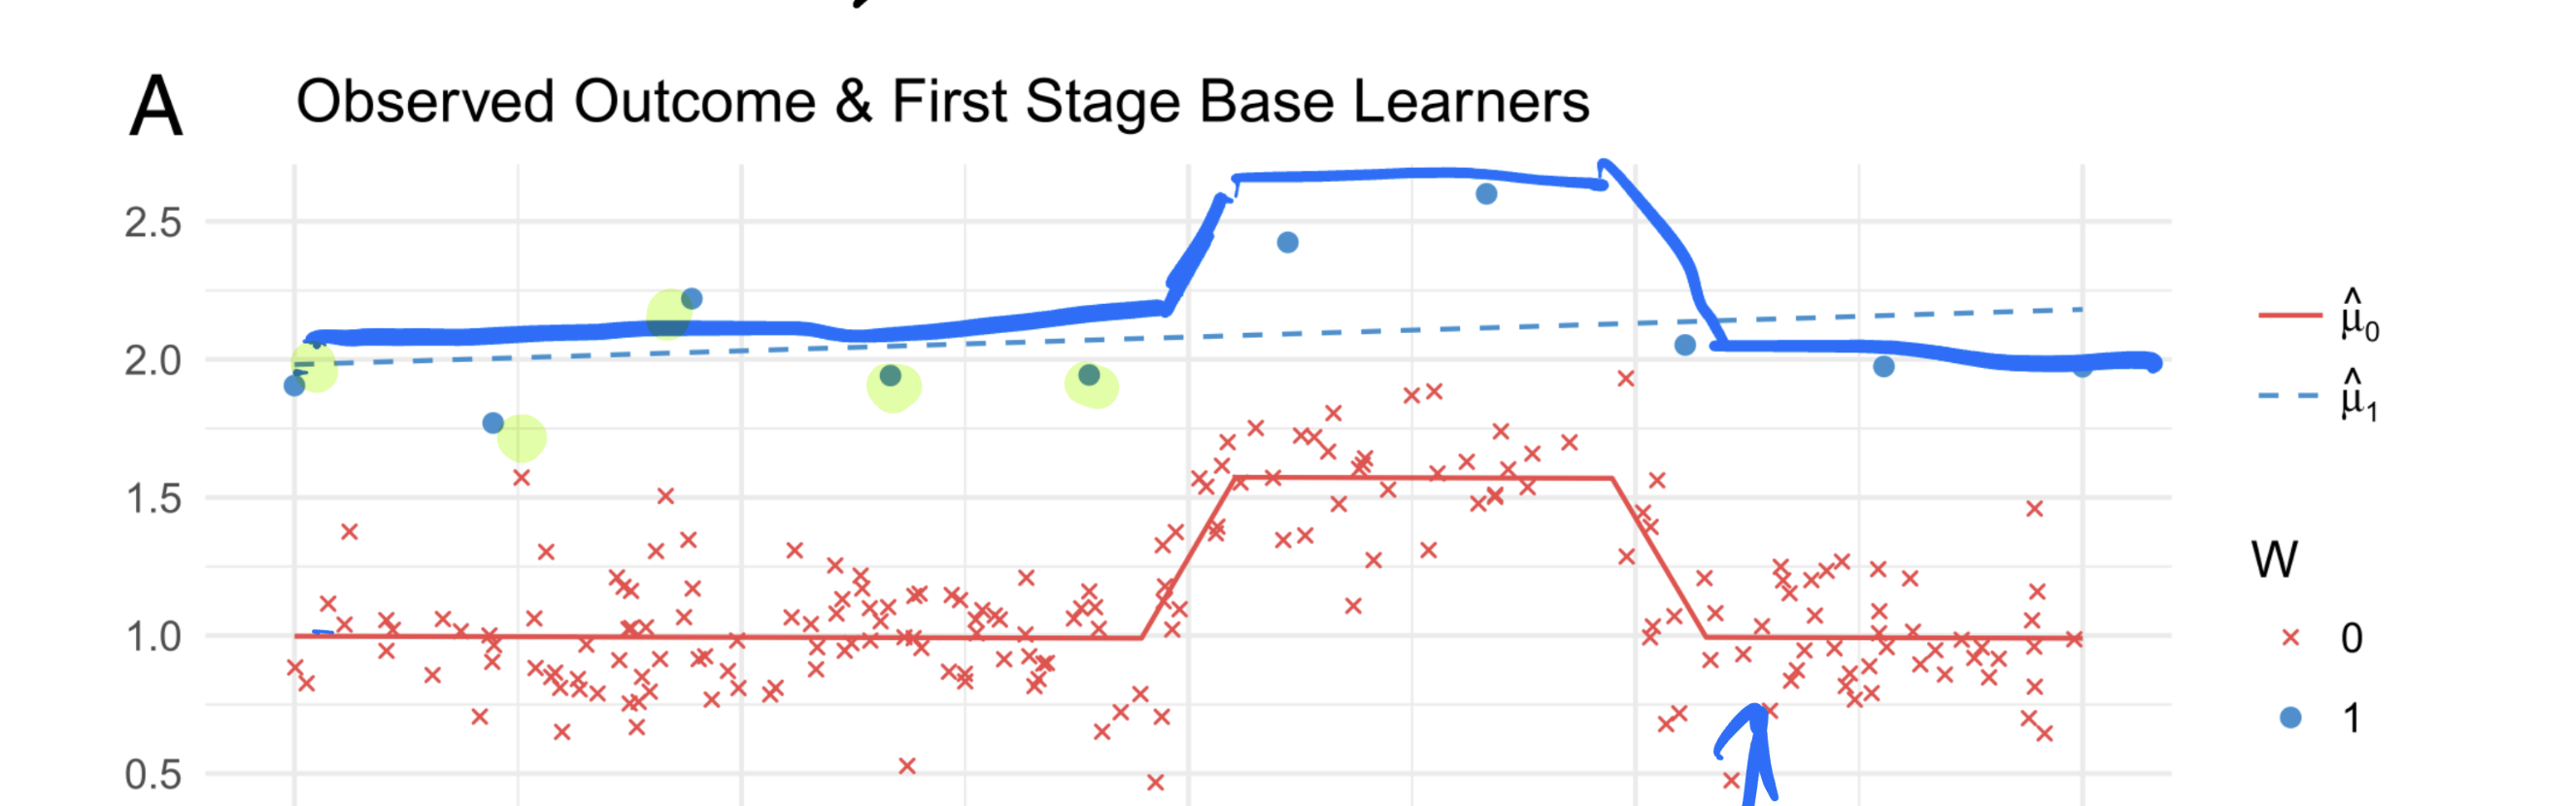
\includegraphics[width=0.78\textwidth]{images/3-12-1}
\end{figure}
Here, we see an example of sparse treatment, where the $x$-learner would fare much better than the $t$-learner.

\begin{definition}[Full $x$-learner]
	Call the above estimator $\hat{\tau}_1$ and do the same thing with roles of $W_i = 1$ and $W_i= 0$ reversed to get $\hat{\tau}_0$. Then put \[
		\hat{\tau}(x) = (1-p) \hat{\tau}_1(x) + p \hat{\tau}_0(x)
	.\] 
	More precisely, put\boxednote{$\tilde{Y}_i$ imputes the missing potential outcome, so its conditional expectation is approximately $\tau(X_i)$. The same logic applies to $\hat{\tau}_1$.}
	\begin{align*}
		\hat{m}_0(\cdot ) &= \mathscr{M}_1 \left[ Y_i \sim X_i, i \in \mathscr{D}_0 \right] \\
		\hat{\tau}_0 (\cdot ) &= \mathscr{M}_2 \left[ \underbrace{Y_i - \hat{m}_0(X_i)}_{\tilde{Y}_i} \sim X_i, i \in \mathscr{D}_1 \right] \\
		\hat{m}_1 &= \mathscr{M}_3\left[ Y_i \sim X_i, i \in \mathscr{D}_1 \right] \\
		\hat{\tau}_1(\cdot ) &= \mathscr{M}_4 \left[ \hat{m}_1(X_i) - Y_i \sim X_i, i \in \mathscr{D}_0 \right] \\
		\hat{\tau}(x) &= (1-p) \hat{\tau}_0(x) + p \hat{\tau}_1(x)
	.\end{align*}

		The simplified $x$-learner is useful with few treatment observations and many controls.
		The full $x$-learner is useful in the opposite regime.
\end{definition}

\begin{definition}[$F$-learner]
	Put
	\begin{align*}
		\tilde{Y}_i &= \frac{W_i Y_i}{p} - \frac{\left( 1-W_i \right)Y_i}{1-p} \\
		&= \begin{cases}
			\frac{Y_i}{p}, \quad W_i = 1 \\ - \frac{Y_i}{1-p}, \quad W_i = 0
		\end{cases}
	.\end{align*} Then use the estimator \[
		\hat{\tau}(\cdot ) = \mathscr{M}\left[ \tilde{Y}_i \sim X_i\text{ for all }i = 1,\ldots,n \right]
	.\] 

	We can check
		\begin{align*}
			\hat{\tau}(x) &= \E\left[\tilde{Y}_i \mid X_i\right]  \\
						  &= \E\left[\frac{W_i Y_i}{p} - \frac{(1-W_i)Y_i}{1-p} \mid X_i\right] \\
						  &= \E\left[\frac{W_iY_i}{p} - \frac{(1-W_i)Y_i}{1-p} \mid X_i, W_i = 1\right] \P\left[W_i = 1\right] \\
						  &\quad + \E\left[\frac{W_iY_i}{p} - \frac{(1-W_i)Y_i}{1-p}\mid X_i, W_i = 0\right] \P\left[W_i = 0\right] \\
						  &= \E\left[\frac{Y_i}{p} \mid X_i, W_i = 1\right] p - \E\left[\frac{Y_i}{1-p} \mid X_i, W_i = 0\right] (1-p) \\
						  &= \E\left[\frac{Y_i(1)}{p} \mid X_i\right] p - \E\left[\frac{Y_i(0)}{1-p} \mid X_i\right] (1-p) \\
						  &= \E\left[Y_i(1) - Y_i(0) \mid X_i\right] = \tau(x)
	.\end{align*}
\end{definition}

\begin{remark}	The $F$-learner is exactly conditionally unbiased. However, if $p$ is close to $0$ or $1$, $\operatorname{Var}\left(\tilde{Y}_i \mid X_i\right)$ could be very large.
\end{remark}

\section{Meta-Learners in Observational Studies}

Let's move from RCTs to observational studies, so we do not randomly assignment treatment, nor do we know $p = \P\left[W_i = 1\right]$.

\begin{notation}	We will now notate
	\[
		e := p = \P\left[W_i = 1\right]  \in (0,1)
	.\] 
\end{notation}

\begin{assumption}
	We wil have standing assumptions of unconfoundedness and overlap.
\end{assumption}

\begin{definition}[Unconfoundedness]
	The treatment is unconfounded if it is independent of potential outcomes, conditional on covariates: \[
		W_i \ind \left( Y_i(0), Y_i(1) \right) \mid X_i
	.\] 
\end{definition}
\begin{definition}[Propensity score]
	Define the propensity score \[
		e(x) := \P\left[W_i = 1 \mid X_i=x\right] 
	.\] In a non-RCT setting, $e(x)$ is generally unknown.

		We say that there is overlap in the study if $e(x) \in (0,1)$ for every $x$.\boxednote{RDD typically does not satisfy overlap, since treatment is determined by whether the running variable crosses the cutoff.}
\end{definition}

The $t$-learner makes sense still, and the estimates $\hat{\tau}_0$, $\hat{\tau}_1$ in the $x$-learner also make sense. Ideally, we would write \[
	\tau(x) = (1-e(x)) \hat{\tau}_0(x) + e \hat{\tau}_1(x)
,\] but we don't know $e(x) = \P\left[W_i = 1 \mid X_i = x\right] $. We can estimate $e$ by regressing $W_i$ on the covariates: \[
	\hat{e}(\cdot ) = \mathscr{M}\left[ W_i \sim X_i, \forall\ i \right]
,\] then estimate \[
	\hat{\tau}(x) = (1-\hat{e}(x)) \hat{\tau}_0(x) + \hat{e}(x) \hat{\tau}_1(x)
.\] 

With the $F$-learner, 
we can put \[
	\tilde{Y}_i = \frac{y_iW_i}{\hat{e}(X_i)} - \frac{Y_i (1-W_i)}{1- \hat{e}(X_i)}
,\] then estimate \[
\hat{\tau}(\cdot ) = \mathscr{M}\left[ \tilde{Y}_i \sim X_i, \forall\ i \right]
.\] 
However, we lose the main appeal of the $F$-learner,\boxednote{We lose the unbiasedness of the $F$-learner because the propensity score $e(x)$ is no longer known (as it was in the RCT) and we estimate it with $\hat{e}$.} in that $\E\left[\tilde{Y}_i \mid X_i\right] \ne \tau(X_i)$. Furthermore, if $e(X_i) \approx 0$ for some $X_i$, then the $F$-learner may blow up.\footnote{In practice, we may use a heuristic to clip $\hat{e} \in [\epsilon,1-\epsilon]$.}

These learners are actually not so great for use in observational studies.
We introduce the Doubly Robust learner.

\begin{remark}	For intuition,
	think of $\tilde{m}_0(\cdot ), \tilde{m}_1(\cdot ), \tilde{e}(\cdot )$ as fixed functions. Then analogously to as in the $t$-learner (with the new addition of debiasing terms), consider \[
		\tilde{Y}_i(\tilde{m}_1, \tilde{m}_0, \tilde{e}) := \tilde{m}_1\left( X_i \right) - \tilde{m}_0(X_i) + \frac{W_i \left( Y_i - \tilde{m}_1(X_i) \right)}{\tilde{e}(X_i)} - \frac{(1-W_i)(Y_i  - \tilde{m}_0(X_i)}{1-\tilde{e}(X_i)}
	.\] 
	The first two terms resemble the $t$-learner, while the second two terms resemble the $F$-learner, but centered around the regression functions.

	Suppose $\tilde{m}_1 = m_1, \tilde{m}_0 = m_0$, but $\tilde{e}$ is arbitrary. Then
		\[
			A_i := m_1(X_i) + \frac{W_i (Y_i - m_1(X_i))}{\tilde{e}(X_i)},
			\qquad
			B_i := m_0(X_i) + \frac{(1-W_i)(Y_i - m_0(X_i))}{1- \tilde{e}(X_i)}.
		\]
		A short conditional-expectation calculation gives
		\[
			\E\left[A_i \mid X_i\right] = m_1(X_i),
			\qquad
			\E\left[B_i \mid X_i\right] = m_0(X_i).
		\]
		Thus $\E\left[\tilde{Y}_i(m_1,m_0,\tilde{e})\right] = \operatorname{CATE}$.

	Now suppose $\tilde{m}_1, \tilde{m}_0$ are arbitrary but the propensity is true in $\tilde{e}= e$.
	Then 
		\[
			\tilde{A}_i := \tilde{m}_1(X_i) + \frac{W_i (Y_i - \tilde{m}_1(X_i))}{e(X_i)},
			\qquad
			\tilde{B}_i := \tilde{m}_0(X_i) + \frac{(1-W_i)(Y_i - \tilde{m}_0(X_i))}{1- e(X_i)}.
		\]
		Again, conditioning on $X_i$ gives
		\[
			\E\left[\tilde{A}_i \mid X_i\right] = m_1(X_i),
			\qquad
			\E\left[\tilde{B}_i \mid X_i\right] = m_0(X_i).
		\]
		Thus $\E\left[\tilde{Y}_i (\tilde{m}_1, \tilde{m}_0, e)\right] = \operatorname{CATE}$.
\end{remark}

If we know perfectly the conditional means of the potential outcomes ($m_1,m_0$) or the propensity score ($e$), then the expectation of $\tilde{Y}_i$ would give the CATE. This motivates the DR-Learner.

\begin{definition}[DR-Learner]
	Put 
	\begin{align*}
		\hat{m}_0(\cdot ) &= \mathscr{M}_1 \left[ Y_i \sim X_i, i: W_i =0 \right] \\
		\hat{m}_1(\cdot ) &= \mathscr{M}_2 \left[ Y_i \sim X_i, i: W_i =1 \right] \\
		\hat{e}(\cdot ) &= \mathscr{M}_2\left[ W_i \sim X_i, \forall\ i \right]\\
		\hat{\tau}(\cdot ) &= \mathscr{M}_4 \left[ \tilde{Y}_i \left( \hat{m}_1, \hat{m}_0 , \hat{e} \right) \sim X_i, \forall\ i \right]
	.\end{align*}
\end{definition}

\begin{aside}	This is better than our other learners for observations studies. The first-order errors cancel, so the remaining bias is second-order: conditioning on $X_i=x$, it is roughly on the scale of
	\[
		\left( \hat{e}(x) - e(x) \right)\left( \left( \hat{m}_1(x) - m_1(x) \right) + \left( \hat{m}_0(x) - m_0(x) \right) \right)
	.\]
\end{aside}

\begin{remark}	There is one remaining problem: overfitting, which we can mitigate by cross-fitting.

	Split the data into two folds $I_1,I_2$ as in cross-validation (each contains treatment and controls). Then we estimate separately on the two folds $\hat{m}_0^{I_1}, \hat{m}_1^{I_1}, \hat{e}^{I_1}$ and $\hat{m}_0^{I_2}, \hat{m}_1^{I_2}, \hat{e}^{I_2}$.
	Then for each $i \in I_1$, we put \[
		\tilde{Y}_i = \tilde{Y}_i \left( \hat{m}_1 ^{I_2}, \hat{m}_0 ^{I_2}, \hat{e}^{I_2} \right)
	,\] 
	and for $i \in I_2$, \[
		\tilde{Y}_i = \tilde{Y}_i\left( \hat{m}_0^{I_1}, \hat{m}_1^{I_1}, e^{I_1} \right)
	.\] 
	Then we pool and estimate \[
		\hat{\tau}(\cdot ) = \mathscr{M}_5\left[ \tilde{Y}_1 \sim X_i, \forall\ i \right]
	.\] 
\end{remark}

The main takeaway is that we can solve lots of prediction problems and combine the results in an intelligent way to solve problems outside prediction.
